\chapter{Experiments and Analysis}

\section{Environment}
All the code for this algorithm was written in Python \pcite{py} and Rust \pcite{rust}. Python was used to read and sanitize the initial dataset, and Rust was used to generate the binary purchase vectors. We opted to use Rust instead of Python for this task because the generation of this vectors has a time complexity of $O(N^2)$ at worst, and therefore may take an order of magnitude longer to run on a slower language such as Python. Python was used for the rest of the tasks, which included the graph generation and clustering, as well as the itemset generation and rule pruning. The following external Python libraries were used to aid development:
\begin{itemize}
\item \texttt{pandas}: Data manipulation.
\item \texttt{numpy}: Data manipulation.
\item \texttt{matplotlib}: Plotting library.
\item \texttt{seaborn}: Plotting library.
\item \texttt{networkx}: Graph generation and plotting.
\item \texttt{markov\_clustering}: Markov Clustering Algorithm.
\end{itemize}

\section{Data Transformation}
\label{sec:algo_data}
Given an itemset $I = \{I_1, I_2,\dots,I_m\}$ and a set of tranactions $T = \{T_1,T_2,\dots\,T_n\}$ such that $T_i \subseteq I$, every transaction $T_i$ will be transformed into a binary purchase vector, as described in Section \ref{sec:binary_purchase_vectors}. An $m \times m$ correlation matrix will then be computed using the Pearson's Correlation Coefficient from the set of binary purchase vectors, composed of the correlation every item has against every other item. A graph $G = (V,E)$ will be constructed from this correlation matrix, such that the vertices $V=I$, and every edge will be the correlation value between the two items it connects. A minimum spanning tree is a sub-graph composed of the \textit{shortest} path connecting all vertices (i.e. the lowest sum of weights), and therefore if we construct our graph from the correlation matrix, the MST would only capture strongly negative and weakly positive relationships only, whereas we want to capture the strongest relationships between products, both negative and positive. Therefore to extract a MST with the strongest associations, the values in the correlation matrix must first be transformed before a graph is constructed from them.

\section{Distance Function}
\label{sec:distance}
As mentioned in Section \ref{sec:binary_purchase_vectors}, the Pearson's Correlation Coefficient is equivalent to the Phi Coefficient ($\phi$) for binary variables, as is the case for our binary purchase vectors. Given $\phi_{ij}$ for items $I_i$ and $I_j$ in the correlation matrix, \pcite{mst_paper} used the distance function
\[
\phi_{ij} = \sqrt{2(1-\phi_{ij})}
\]
to transform their correlation matrix. Given that we are using the Pearson's Correlation Coefficient that gives us a correlation score in the interval [-1,1], this equation is not suitable for us as it discards the strongly negative associations by outputting a larger weight (e.g. a correlation score of -1 would be transformed to 2) which would not be captured in the MST. Therefore, we modify the equation to be
\[
\phi_{ij} = \sqrt{2(1-|\phi_{ij}|)}
\]
allowing us to capture both positive and negative associations alike. Figure \ref{fig:distance_function} illustrates the effect of our distance function, where the stronger the correlation of the input, the lower the output. Given that our initial correlation values were bound to the interval $[-1,1]$, the output of the distance function is similarly bound to the interval $[0, \sqrt{2}]$.
\begin{figure}[H]
\centering
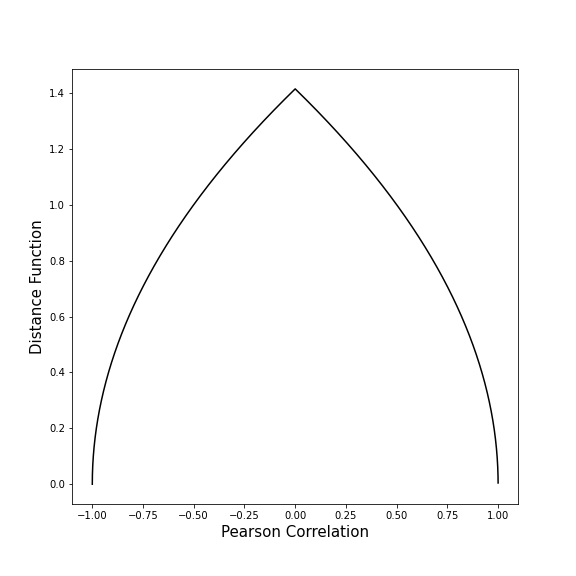
\includegraphics[scale=0.4]{distance_function}
\label{fig:distance_function}
\caption{The effect of the distance function $\sqrt{2(1-|x|)}$}
\end{figure}
\noindent Once the correlation matrix has been transformed via this function, the graph $G=(V,E)$ can be constructed.



\section{Dataset Pre-Processing}
The dataset used in this study is the sales data of $4,152,919$ transactions and $39$ unique product categories from a chain of Brazilian gas-station stores \pcite{data_source}.
Each row in the dataset represents the purchase of a specific product as part of a transaction - and as such, each row corresponds to the following columns:
\begin{itemize}
\item Company Code
\item Order Number
\item Employee
\item Product
\item Product Category
\item Client
\item Sale Date Time
\item Product Cost
\item Discount Amount
\end{itemize}
All personal and corporate names were exchanged for fictitious names by the author of the dataset in order to preserve the anonymity of those whose who could have otherwise been identified through the dataset.
% columns_to_export = ['product', 'product_category', 'client_city', 'discount_amount', 'basket_id']
Only the Product, Product Category, Client City and Discount Amount columns were retained for the purposes of our algorithm, the rest were discarded.
Before employing the dataset, sanitary procedures were carried out to ensure that the dataset was error-free and in a format suitable for graph generation. The steps have been detailed below.

\begin{enumerate}
\item \textbf{Transaction Identifier}\\
The \textit{Order Number} field showed discrepancies, where a given order number could reference distinct transactions in different stores and cities, and at different dates and times. 
This could be due to the stores maintaining their own order numbers, and also because the order numbers may reset after a predetermined limit.
A unique transaction identifier - named \texttt{basket\_id} - was created by concatenating the order number and the date, thereby mitigating the occurrence of a identifier that references multiple transactions.

\item \textbf{Binary Purchase Vector transformation}\\
The dataset was then transformed such that each transaction was represented by a binary purchase vector - as described in Section \ref{sec:algo_data} - wherein each column represents a product category. The product categories were chosen for the graph representation over the products themselves as it would give a more generalized view on the associations between them, and the categories themselves were deemed specific enough that they would not be parent to children of significant variance.
\end{enumerate} 
\begin{figure}[H]
\centering
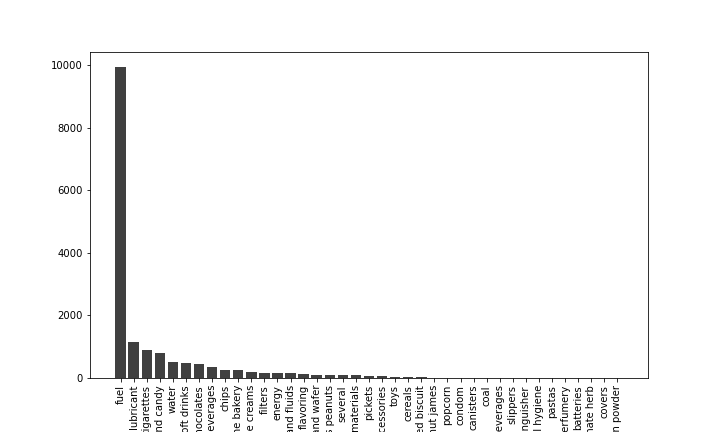
\includegraphics[scale=0.5]{category_dist}
\caption{Category Distribution}
\label{fig:cat_dist}
\end{figure}
The metrics used to assess the association rules - support, lift and confidence - are based on the proportional presence of a given itemset in the transactions. Since our dataset is from a gas-station store chain, fuel products dominate the transactional presence by a significant factor. Figure \ref{fig:cat_dist} highlights the disparity between the presence of \textit{fuel} products and the others, with \textit{fuel} being present in $99.28\%$ of all transactions. To avoid the association rules being dominated by the \textit{fuel} category - which should inherently understood to be a key product for gas stations - the fuel category was purged from the dataset, reducing the dataset to $1,362,617$ transactions.
The correlation matrix for the $38$ remaining product categories was then computed using Pearson's Correlation Coefficient, and is illustrated in Figure \ref{fig:correlation}. Since the correlation matrix is known to be diagonally symmetrical, only the values below the diagonal have been illustrated.
\begin{figure}[H]
\centering
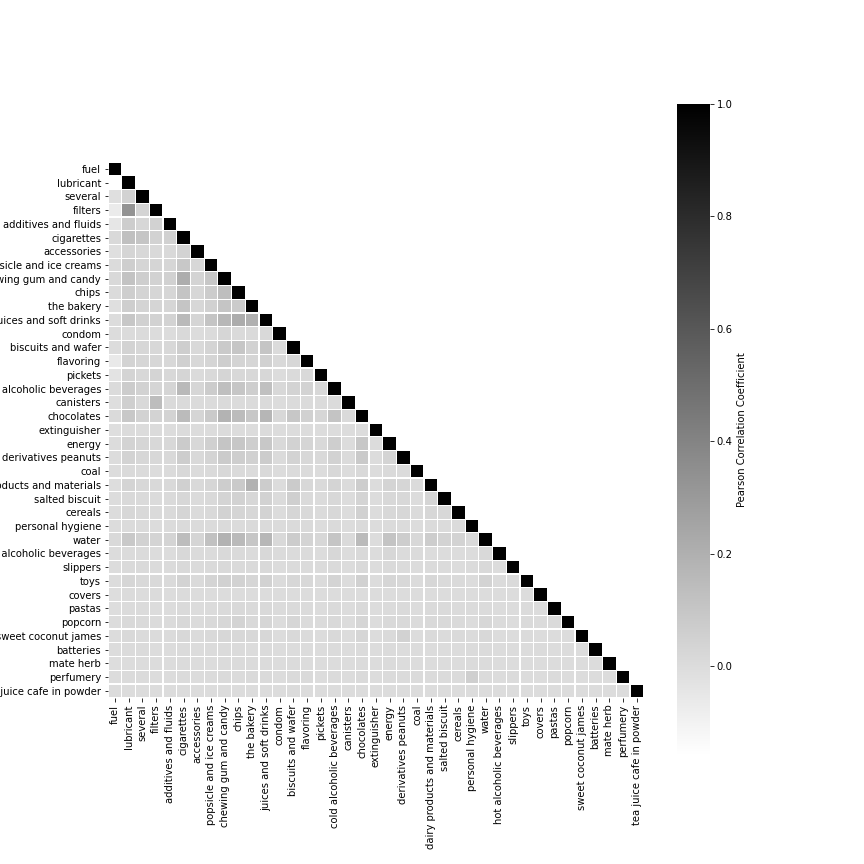
\includegraphics[scale=0.4]{correlation}
\caption{Correlation Matrix from Binary Purchase Vectors}
\label{fig:correlation}
\end{figure}


\section{MST Generation}
As described in \ref{sec:distance}, the distance function $\sqrt{2(1-|\phi_{ij}|)}$ was then applied to the correlation matrix to transform the values such that the strongest associations have the lowest values. The graph $G=(V,E)$ was then constructed such that the vertices $V$ represent the product categories, and the weights of the edges $E$ are the transformed correlation values between the vertices the edges connect. The minimum spanning tree was then extracted from this graph using Kruskal's algorithm. Both the complete graph and the MST are illustrated in Figure \ref{fig:graph_mst}. The value of each node is an integer, which corresponds to the index of the product category in the binary purchase vector dataset. The length of each edge is directly proportionate to its weight, such that the greater the weight, the greater the length of the edge.
\begin{figure}[H]
\centering
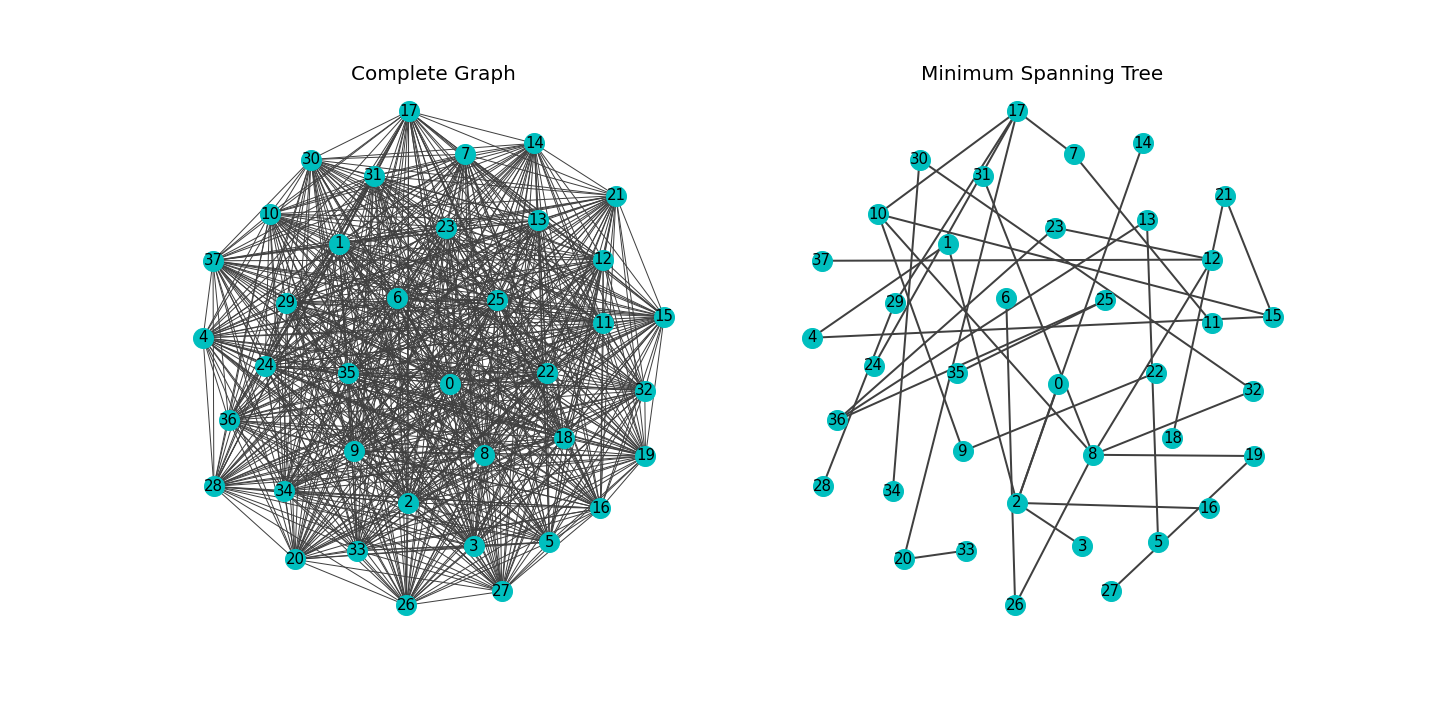
\includegraphics[scale=0.31]{graph_and_mst_no_fuel}
\caption{Product Category Graph and MST}
\label{fig:graph_mst}
\end{figure}

\section{Markov Clustering}
\begin{figure}[H]
\centering
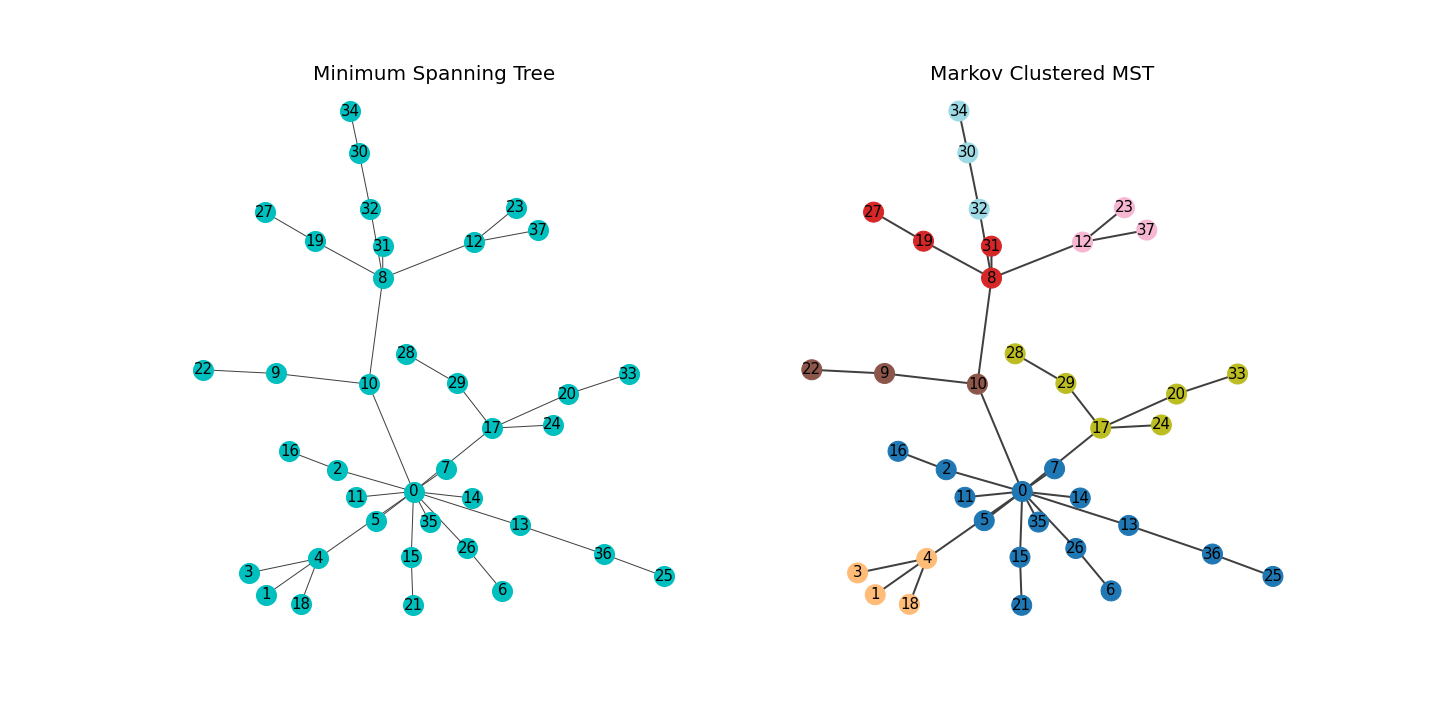
\includegraphics[scale=0.31]{mst_clustered_no_fuel2}
\caption{MST before and after Markov Clustering}
\label{fig:clustered}
\end{figure}
The MST was then clustered using the Markov Clustering algorithm. To identify the most modular clustering configuration, we implemented the algorithm several times with inflation scores between 1.5 and 2.5 (inclusive) at increments of 0.1. In doing so, we discovered that an inflation score of 1.6 resulted in the most optimal modularity. The Markov Clustering configuration produced using this inflation score was therefore chosen, and the results of this clustering are illustrated in Figure \ref{fig:clustered}. Note that while the disposition of nodes differs from that illustrated in Figure \ref{fig:graph_mst}, the nodes and the edge weights are the same.
The Markov Clustering algorithm segmented the nodes into 8 distinct clusters.
Figure \ref{fig:cluster_named} illustrates the names of the product categories in each cluster, color-coded in accordance with the MSTs in Figure \ref{fig:clustered}. Observing the groupings produced by the MCL algorithm, we can see that with the exception of the largest cluster in blue, the groupings do have an underlying similarity (e.g. \texttt{\{biscuits and wafer, salted biscuit, tea juice cafe in powder\}}).

\begin{figure}[H]
\centering
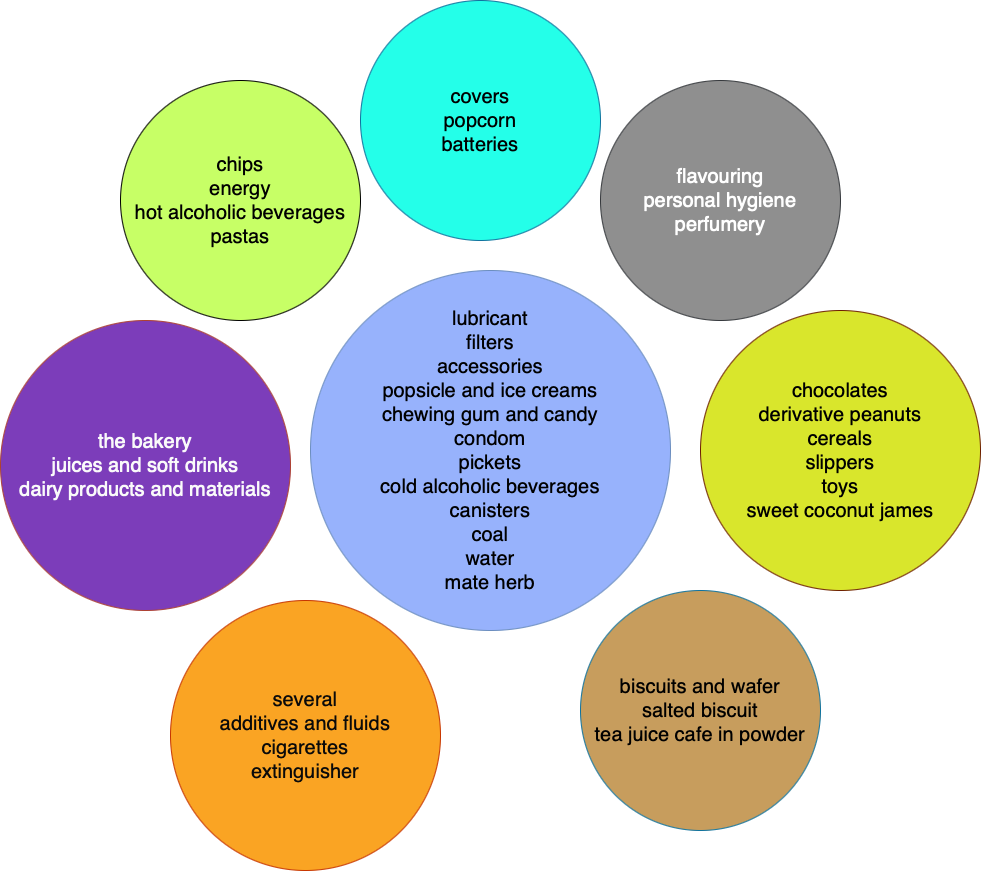
\includegraphics[scale=0.3]{cluster_named}
\caption{Product categories by cluster}
\label{fig:cluster_named}
\end{figure}


\section{Comparison of \algo\ and Apriori Algorithm}
Once the MST was clustered, we used both the \algo\ and the Apriori Algorithm to generate rules for our dataset, with the support constraint at $0.1\%$ and the confidence constraint at $25\%$. Given these constraints, the Apriori algorithm generated $1,222$ rules, and the \algo\ generated $123$ bi-cluster rules as well as $60$ intra-cluster rules, totalling $183$ rules.\\
\\\\\textbf{Apriori Rules}\\
We present the first 5 rules generated by the Apriori Algorithm, ranked by highest support.

\begin{longtable}
{@{}llllll@{}}\toprule Antecedent& Consequent& Support& Confidence& Lift& Type\\*\midrule\endfirsthead\endhead
\{chewing gum and candy\} & \{cigarettes\} & 0.0726 & 0.2986 & 1.0985 & Apriori\\
\{cigarettes\} & \{chewing gum and candy\} & 0.0726 & 0.2671 & 1.0985 & Apriori\\
\{water\} & \{chewing gum and candy\} & 0.0473 & 0.3052 & 1.2554 & Apriori\\
\{filters\} & \{lubricant\} & 0.0468 & 0.9381 & 2.6850 & Apriori\\
\{chocolates\} & \{chewing gum and candy\} & 0.0435 & 0.3117 & 1.2820 & Apriori\\
\midrule\caption{Apriori Rules}\label{tab:apri_rules}\end{longtable}

\noindent \textbf{\algo\ Rules}\\
Similarly, we present the first 5 rules generated by the \algo, ranked by highest support. The type of rule has also been annotated (i.e. bi-cluster or intra-cluster).

\begin{longtable}
{@{}llllll@{}}\toprule Antecedent& Consequent& Support& Confidence& Lift& Type\\*\midrule\endfirsthead\endhead
\{chewing gum and candy\} & \{cigarettes\} & 0.0726 & 0.2986 & 1.0985 & bi-cluster\\
\{cigarettes\} & \{chewing gum and candy\} & 0.0726 & 0.2671 & 1.0985 & bi-cluster\\
\{water\} & \{chewing gum and candy\} & 0.0473 & 0.3052 & 1.2554 & intra-cluster\\
\{filters\} & \{lubricant\} & 0.0468 & 0.9381 & 2.6850 & intra-cluster\\
\{chocolates\} & \{chewing gum and candy\} & 0.0435 & 0.3117 & 1.2820 & bi-cluster\\
\midrule\caption{\algo\ rules}\label{tab:arm_rules}\end{longtable}

\noindent \textbf{Analysis}\\
We observe that there is a $100\%$ overlap between the top five rules generated by the Apriori algorithm and the \algo. The $100\%$ overlap stands true for up until the first $13$ rules for both algorithms, after which a decline can be observed. 
\begin{figure}[H]
\centering
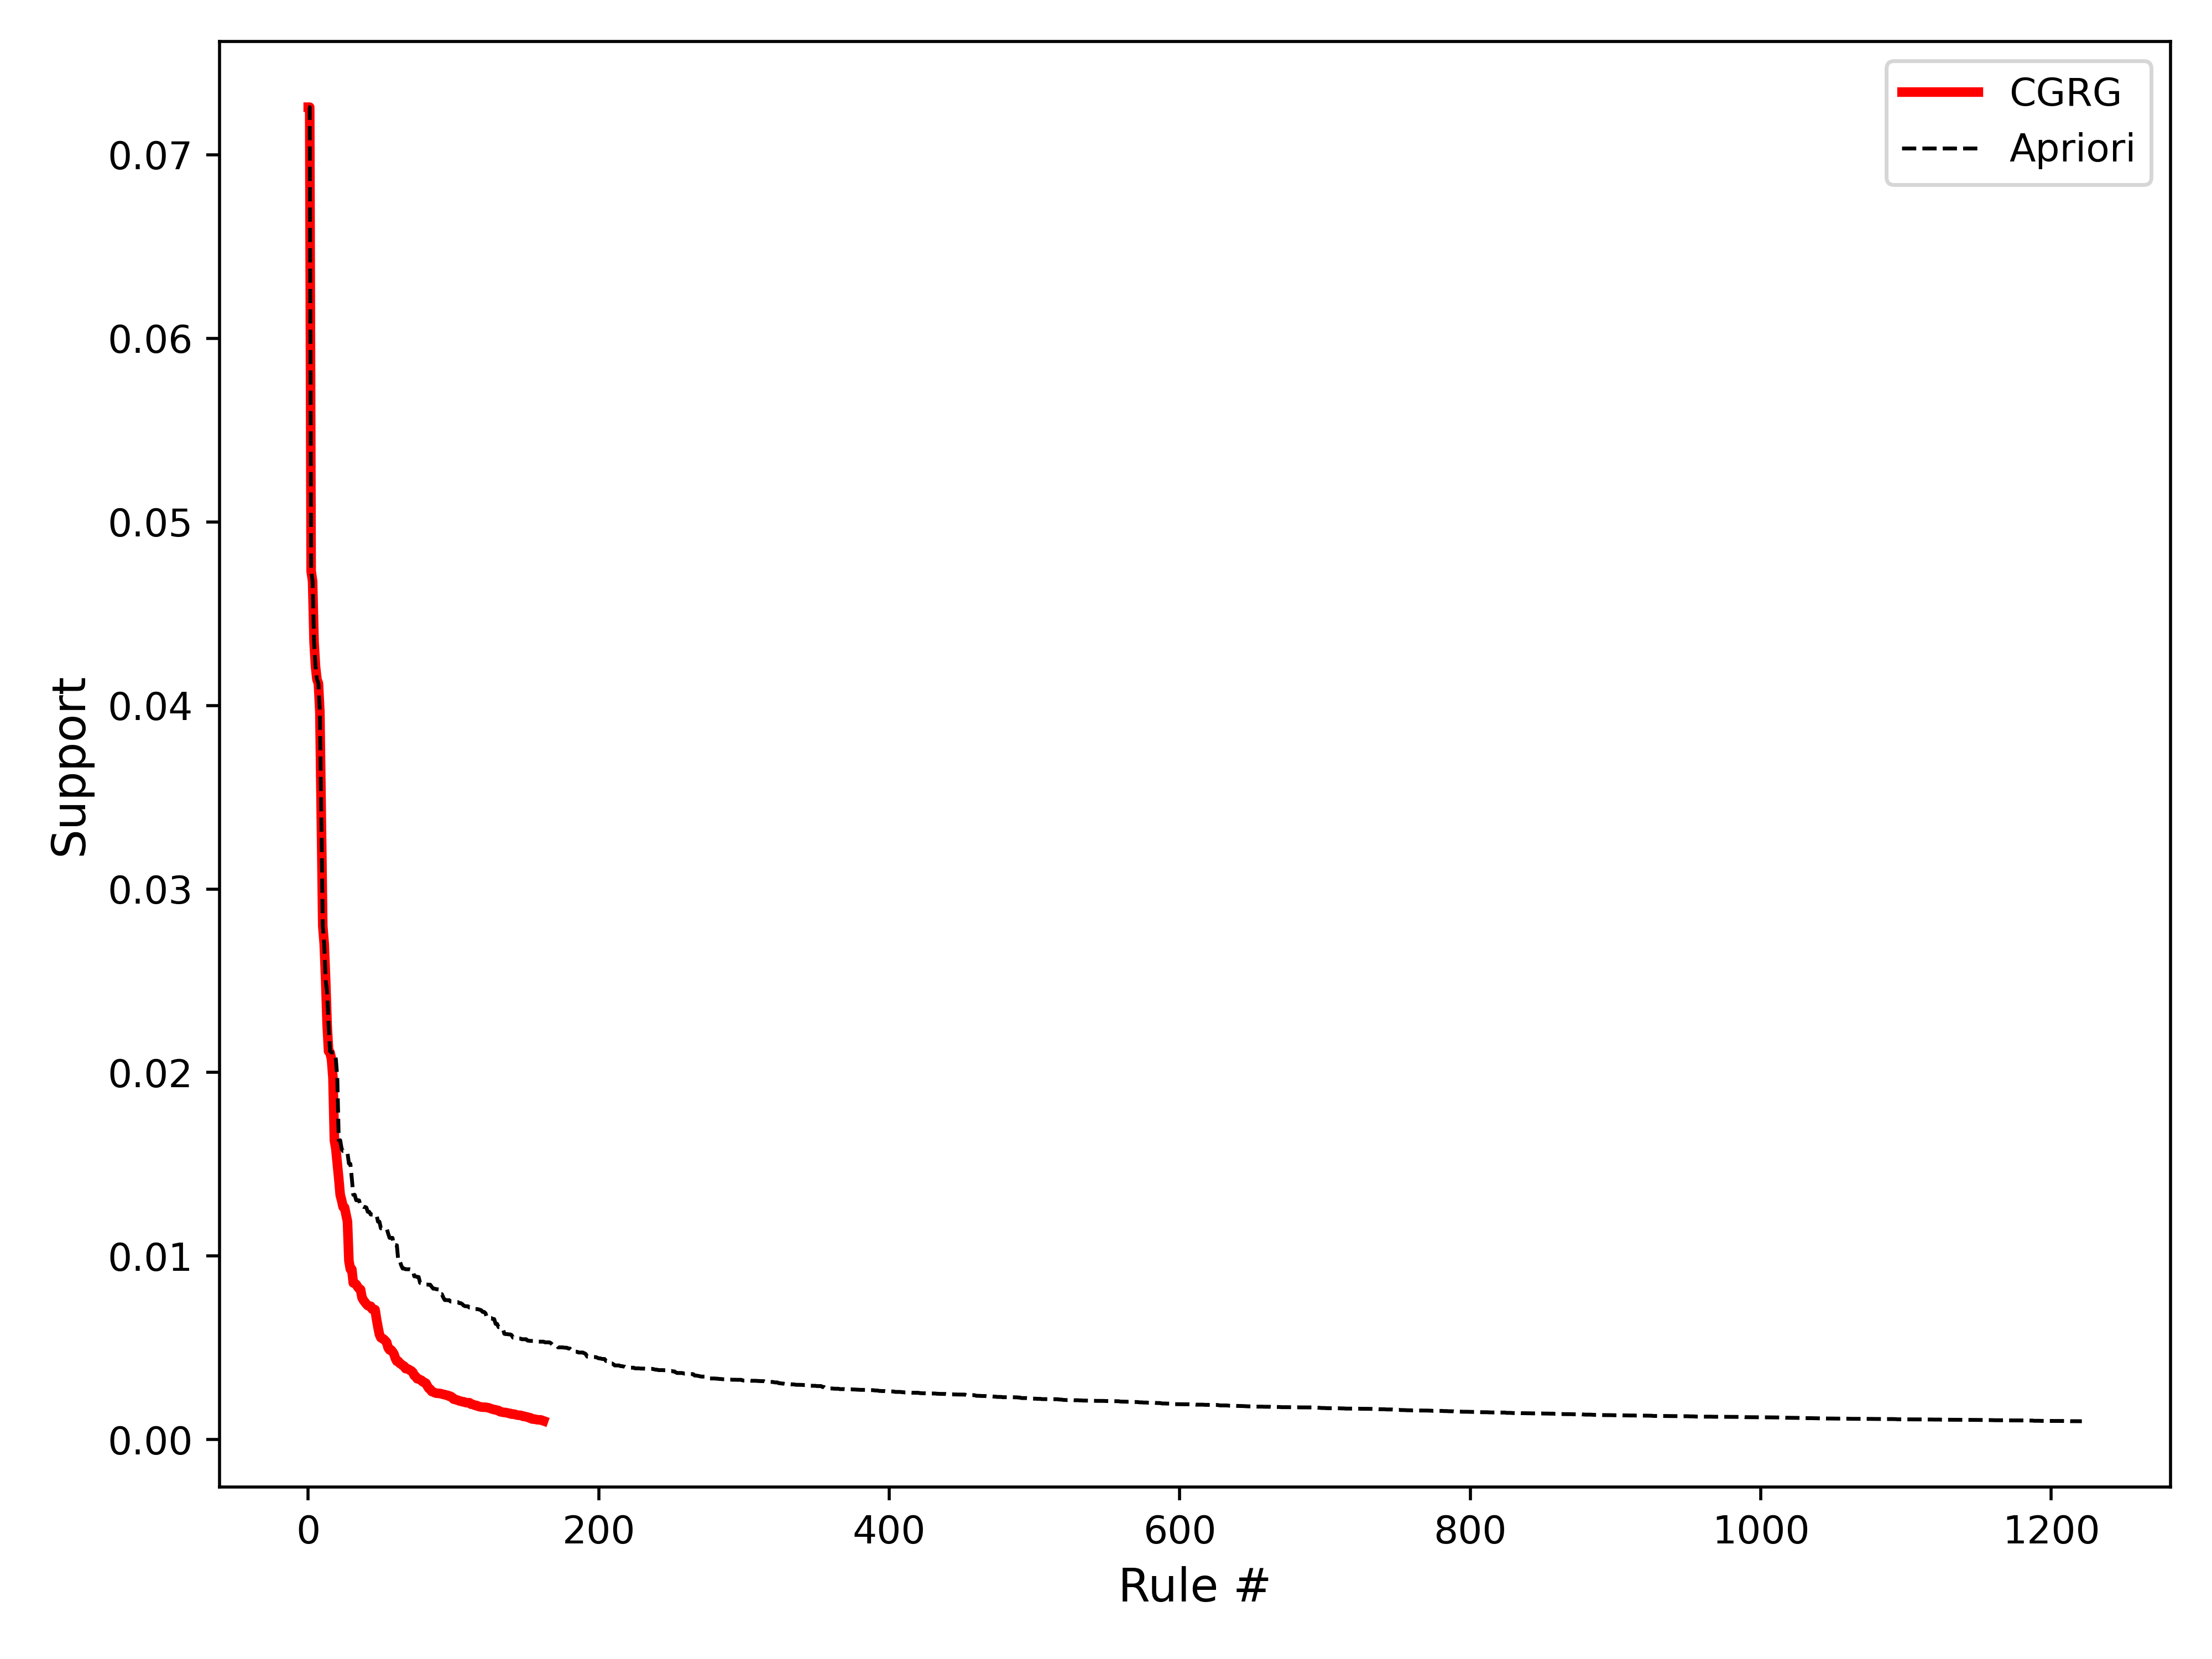
\includegraphics[scale=0.65]{ruleset_support}
\caption{Ranked supports for both the \algo\ and Apriori Algorithm}
\label{fig:rule_support}
\end{figure}
\noindent Figure \ref{fig:rule_support} illustrates the support values for the $x^{th}$ rule for both the \algo\ and Apriori when they are sorted by the highest support score to the lowest. 
We can observe that when provided with the same support and confidence constraints, the Apriori algorithm produces far greater rules, whereas the \algo\ algorithm captures mostly the those rules that have a relatively higher support, with the exception being at the elbow of both curves, where the \algo\ algorithm captured rules with a lower support than the Apriori algorithm.\\
We can infer from this figure that the \algo\ algorithm captures the strongest rules present in the Apriori ruleset, which leads us to theorize that \textit{rules where the itemsets each originate from the same cluster are likelier to have a higher support score than those which don't}. In other words, given clusters $A$ and $B$, and subsets of any given cluster $cl_i$ and $cl_j$, rules which follow:
\[
cl_i \rightarrow cl_j;\;\;\;cl_i \subset A, \;\;\; (cl_j \subset B \;|\; cl_j \subset A)
\]
are likelier to have a higher support score than rules whose antecedent and/or consequent are composed of items from multiple clusters.
To further reinforce this theory, we present the averages of the support, confidence and lift scores generated by both algorithms:
\begin{longtable}
{@{}llll@{}}\toprule Algorithm& Mean Support& Mean Confidence& Mean Lift\\*\midrule\endfirsthead\endhead
Apriori & 0.0034& 0.3737& 1.9096\\
\algo\ & 0.0075& 0.3683& 1.8855\\
\midrule\caption{Averages for both algorithms}\end{longtable}
\noindent We can see that while the mean confidence and lift scores from the Apriori algorithm are only marginally higher those from the \algo\ algorithm, the mean support for the \algo\ algorithm is significantly greater than that of the Apriori algorithm by a factor of approximately $2.2$, indicating that the composition of the rules generated by the \algo\ algorithm is far more concentric in high-value rules than the Apriori generated ruleset.
\begin{figure}[H]
\centering
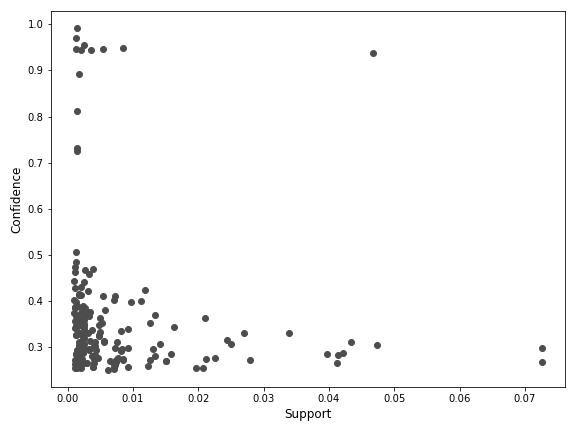
\includegraphics[scale=0.65]{confsupp}
\caption{Relationship between confidence and support for \algo}
\label{fig:confsupp}
\end{figure}
Figure \ref{fig:confsupp} illustrates the relationship between the confidence and support for the rules generated by the \algo\ algorithm.
The majority of rules generated are concentric around the support and confidence constraints of $0.001$ and $0.25$ respectively. The outliers indicate a negative relationship between the two metrics: the rules with the highest confidence had a relatively low support, and vice versa.

As \pcite{lift} argued, the \textit{lift} score may be a better metric to assess the value of a rule than support or confidence. Figure \ref{fig:rule_lift} illustrates the lift values for the $x^{th}$ rule for both the \algo\ and Apriori when they are sorted by the highest lift score to the lowest. The image has been zoomed to illustrate only the first $183$ rules (the length of the \algo\ ruleset) to further illustrate the disparity at the elbows of the curves.
\begin{figure}[H]
\centering
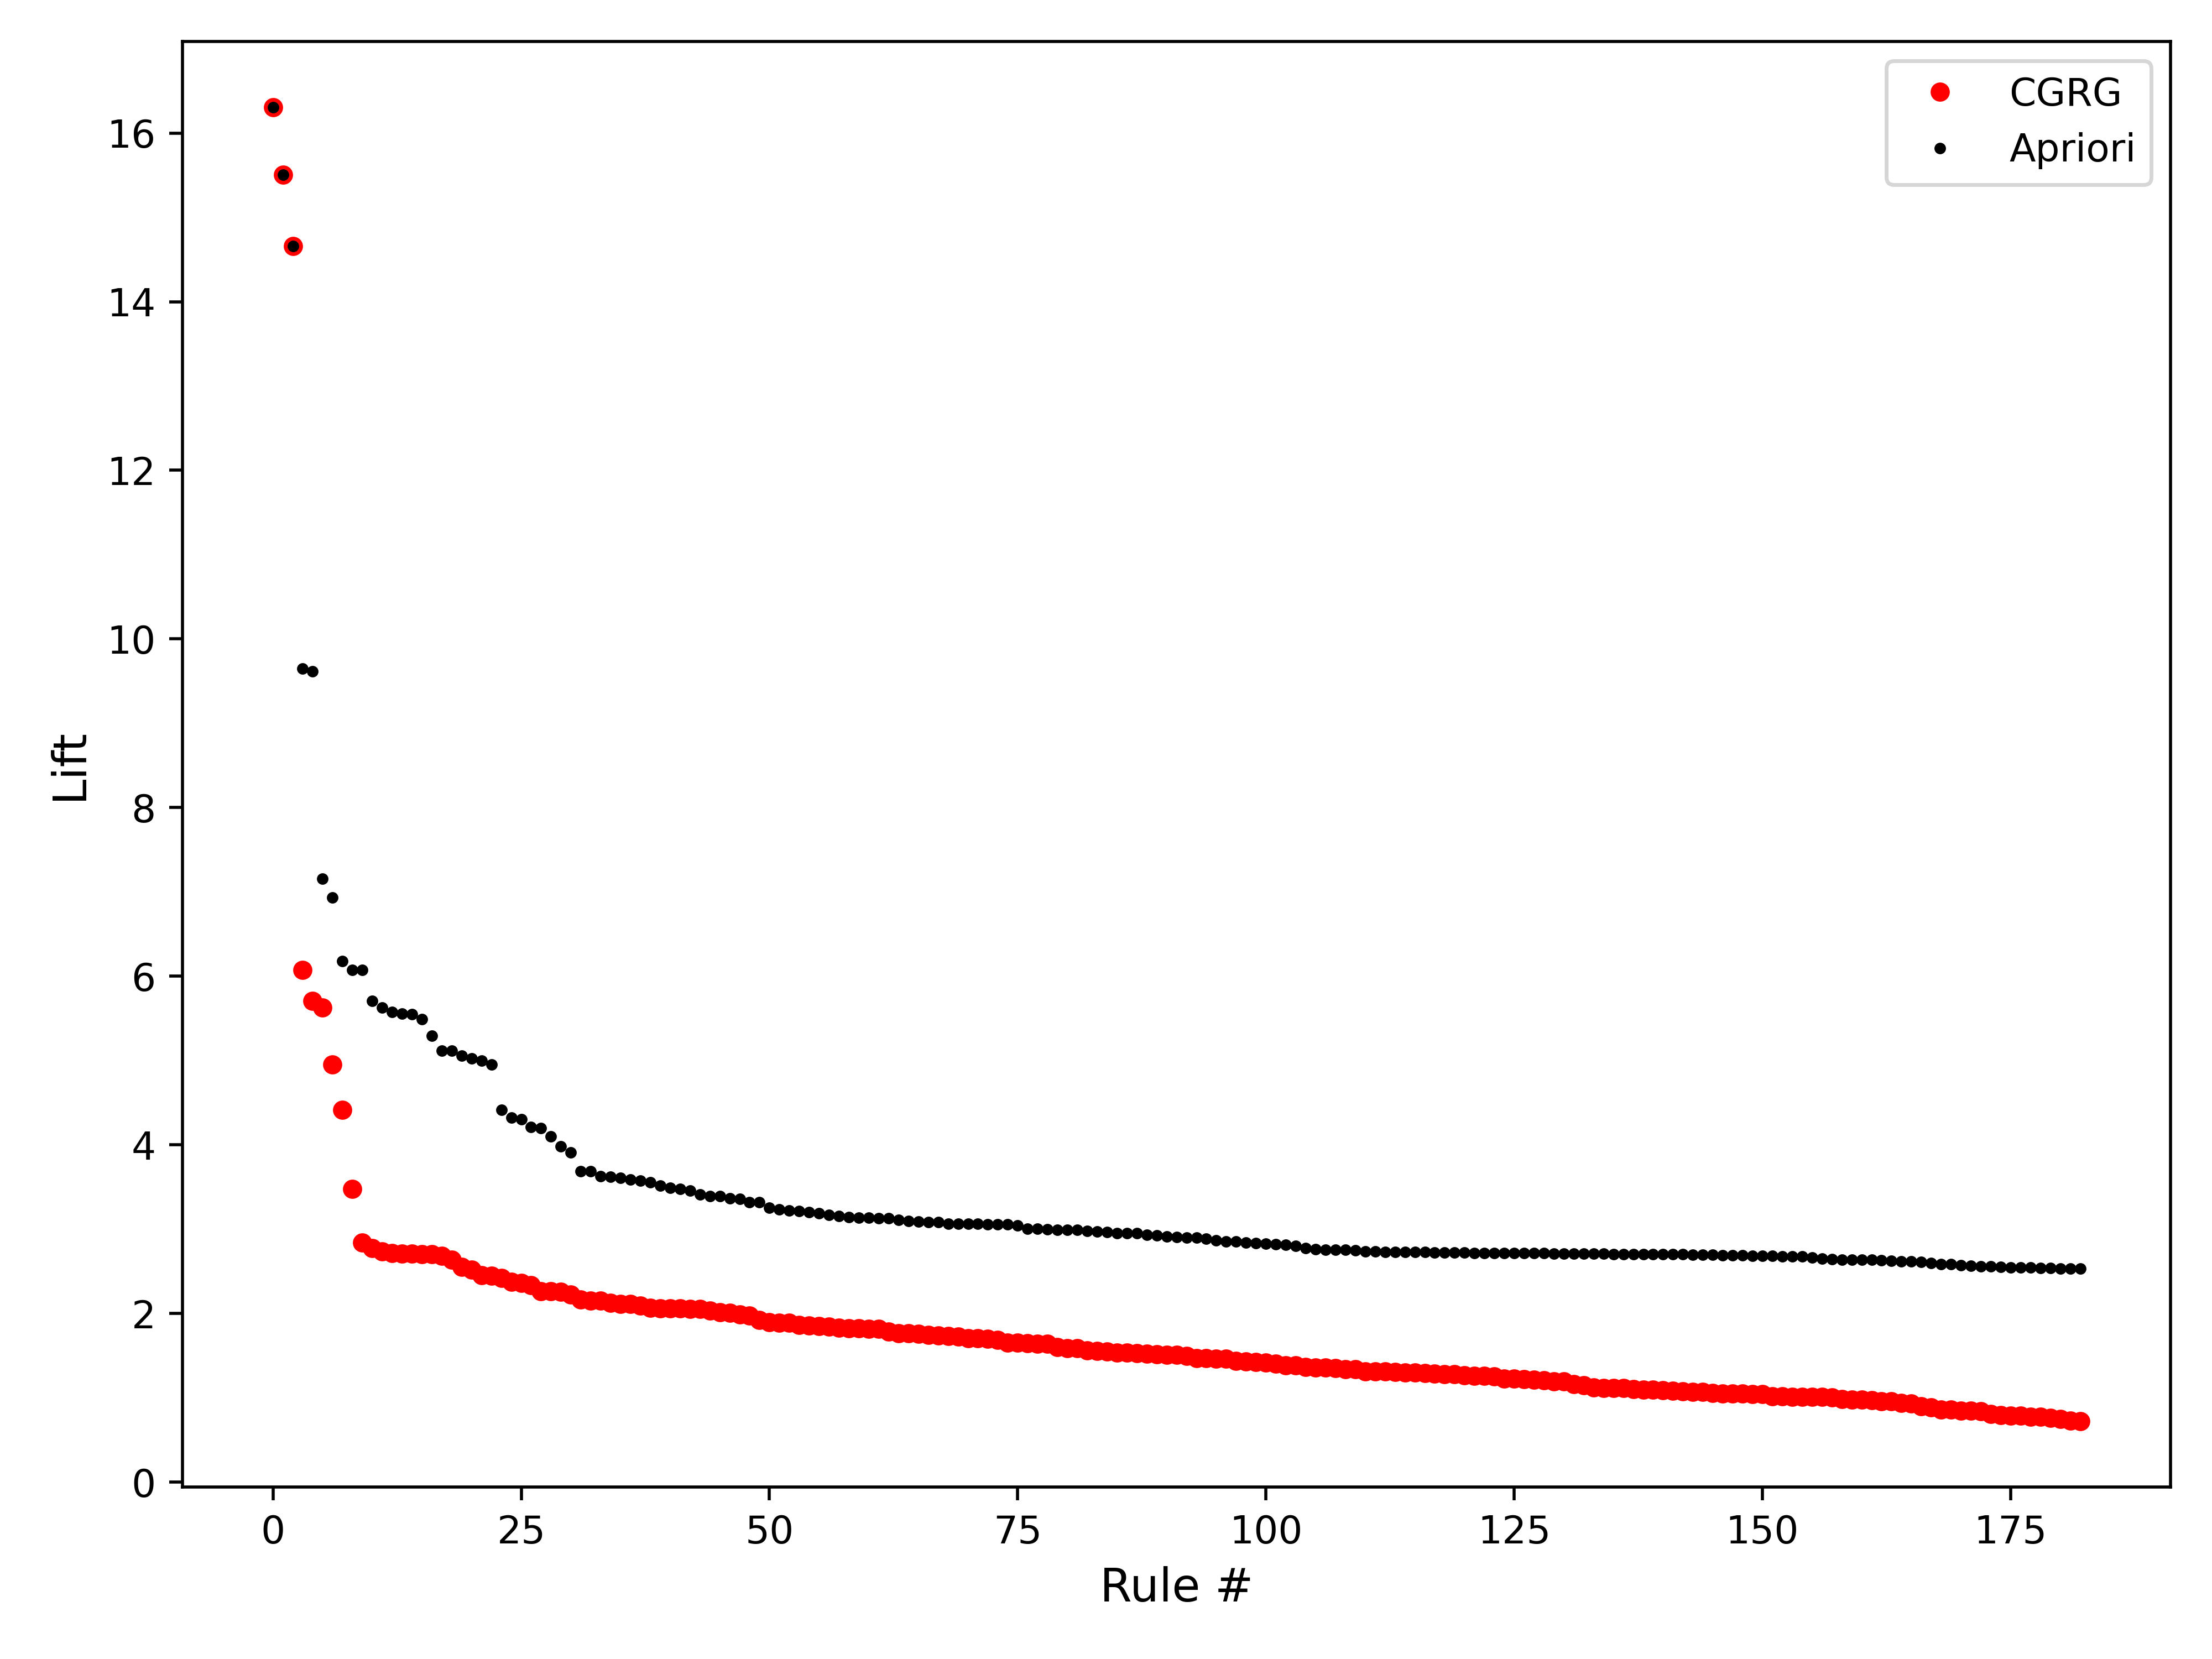
\includegraphics[scale=0.65]{ruleset_lift_zoom}
\caption{Ranked lift scores for both the \algo\ and Apriori Algorithm}
\label{fig:rule_lift}
\end{figure}
The figure is similar to the ranked support scores in Figure \ref{fig:rule_support}, however the disparity at the elbow of the curves is much greater. This may indicate that the antecedent may give a higher rise to the confidence of a rule when the composition of the antecedent and/or the consequent consists of items from multiple clusters. To illustrate the high lift rules our algorithm has failed to capture, the first five multi-element rules generated by both algorithms and ranked by lift scores have been detailed below:

\begin{longtable}
{@{}llllll@{}}\toprule Antecedent& Consequent& Support& Confidence& Lift& Type\\*\midrule\endfirsthead\endhead
\{canisters,lubricant\} & \{filters\} & 0.0014 & 0.8128 & 16.3071 & Apriori\\
\{canisters\} & \{filters,lubricant\} & 0.0014 & 0.7250 & 15.5054 & Apriori\\
\{canisters\} & \{filters\} & 0.0014 & 0.7308 & 14.6611 & Apriori\\
\{chips,filters\} & \{juices and soft drinks,lubricant\} & 0.0011 & 0.3528 & 9.6487 & Apriori\\
\{filters,the bakery\} & \{juices and soft drinks,lubricant\} & 0.0011 & 0.3515 & 9.6143 & Apriori\\
\midrule\caption{Apriori Rules ranked by Lift}\label{tab:apri_lift}\end{longtable}

\begin{longtable}
{@{}llllll@{}}\toprule Antecedent& Consequent& Support& Confidence& Lift& Type\\*\midrule\endfirsthead\endhead
\{lubricant,canisters\} & \{filters\} & 0.0014 & 0.8128 & 16.3071 & intra-cluster\\
\{canisters\} & \{lubricant,filters\} & 0.0014 & 0.7250 & 15.5054 & intra-cluster\\
\{canisters\} & \{filters\} & 0.0014 & 0.7308 & 14.6611 & intra-cluster\\
\{filters,water\} & \{lubricant,chewing gum and candy\} & 0.0020 & 0.3525 & 6.0734 & intra-cluster\\
\{lubricant,pickets\} & \{filters\} & 0.0013 & 0.2844 & 5.7052 & intra-cluster\\
\midrule\caption{\algo\ Rules ranked by Lift}\end{longtable}
The first three rules with the highest lift are present in the rulesets of both algorithms, however the \algo\ did not capture the fourth and fifth rule in Table \ref{tab:apri_lift}. This further reinforces our belief that the structural constraints of the rules the \algo\ algorithm produces impedes the algorithm from generating the rules such as those present in the Table \ref{tab:apri_lift}.